\documentclass[12pt]{article}


\usepackage[utf8]{inputenc}
\usepackage[a4paper,top=3cm,bottom=2cm,left=3cm,right=3cm,marginparwidth=1.75cm]{geometry}
\usepackage[nodayofweek]{datetime}
\usepackage{tabularx}
\usepackage[small]{titlesec}
\usepackage{graphicx}
\usepackage{tabularx}
\usepackage{amsmath}
\usepackage{fancyvrb}
\newcolumntype{L}[1]{>{\raggedright\arraybackslash}p{#1}}
\newcolumntype{C}[1]{>{\centering\arraybackslash}p{#1}}
\newcolumntype{R}[1]{>{\raggedleft\arraybackslash}p{#1}}

\begin{document}

\begin{titlepage}
    \begin{center}
        \huge{\bfseries  Tribhuvan University}\\
        \Large{Institute of Engineering}\\
        \huge{ \bfseries  Pulchowk Campus}\\[3.2cm]


        \textsc{\Large Digital Signal Analysis and Processing}\\[-0.5cm]
        \line(1,0){400}\\
        \huge{\bfseries Lab 5}\\
        \huge{z Transformations}
        \line(1,0){400}\\


        \textsc{\Large Submitted by:}\\
        \Large Bishal Katuwal\\ \large 075BCT028\\    [0.85cm]

        \textsc{\Large Submitted to:}\\\
        \large Department of Electronics and Computer Engineering\\Pulchowk Campus\\    [0.85cm]
        
        \textsc{\Large Submitted on:}\\
        \today
        
    \end{center}
\end{titlepage}
\pagebreak
% ===============================================================
\paragraph{Title\\}
z-Transformation
\paragraph{Background Theory\\}


In Laplace transform, a function of time is converted into a function of frequency. 
The z-transform can be thought of as a discrete-time version of the Laplace transform. 
Using the complex variable z and by applying the z-transform to a sequence of data points, 
an expression is created that allows us to perform frequency-domain analysis of discrete-time signals.

With the z-transform, we can create transfer functions for digital filters, 
and we can plot poles and zeros on a complex plane for stability analysis. 
The inverse z-transform allows us to convert a z-domain transfer function into a difference equation 
that can be implemented in code written for a microcontroller or digital signal processor.

The relationship between a discrete-time signal x[n] and its one-sided z-transform X(z) is expressed as follows:
\begin{equation}
        X(z) = \sum_{n=0}^{\inf} x(n)z^{-n}
\end{equation}
\subparagraph{MATLAB implementation\\}
In MATLAB, we use {\bfseries signal} package for z- transformation. 
Some functions involved in z-transform are: 
\begin{itemize}
    \item {\bfseries zplane} : Plot the poles and zeros on a complex plane.
    \item {\bfseries sos2zp} : Convert series second-order sections to zeros, poles, and gains (pole residues).
    \item {\bfseries ss2zp} : Converts a state space representation to a set of poles and zeros; K is a gain associated with the zeros.
    \item {\bfseries tf2zp} : Convert transfer functions to poles-and-zero representations.
    \item {\bfseries zp2sos} : Convert filter poles and zeros to second-order sections.
    \item {\bfseries zp2ss} : Conversion from zero / pole to state space.
    \item {\bfseries zp2tf} : Converts zeros / poles to a transfer function.
    \item {\bfseries czt} : Chirp z-transform
\end{itemize}
\pagebreak
\paragraph{Activity\\}
Locate the position of zeroes and poles in the z plane.
\begin{enumerate}
    \item \begin{verbatim}
        h[n] = [1, 2, 3.4, 6.3, 0.7, 2]
    \end{verbatim}
    \begin{Verbatim}[frame=single]
pkg load signal
f=[1,2,3.4,6.3,0.7,2]
F = czt(f)
zplane(F)
title('075BCT028')
    \end{Verbatim}
    \begin{figure}[h!]
        \centering
        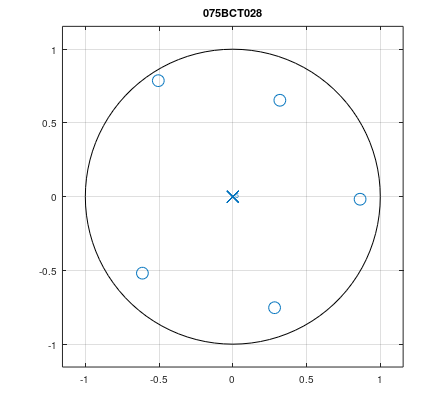
\includegraphics{labss/Lab5_1.PNG}
        \caption{Poles and zeroes of  h[n] = [1, 2, 3.4, 6.3, 0.7, 2]}
    \end{figure}
    \item \begin{equation}
        H(z) =  \frac{1 - 0.4 z^{-1} + 0.2 z^{-3} + 0.77 z^{-5} }{ 0.78 + 1.5 z^{-1} +z^{-4} + 8.2 z^{-5} } \nonumber
    \end{equation}

    \begin{Verbatim}[frame=single]
        pkg load signal
        num = [1 -0.4 0 0.2 0 0.77]
        dem =  [0.78 1.5 0 0 1 8.2]
        zplane(num,dem)
        title('075BCT028')
            \end{Verbatim}
            \begin{figure}[h!]
                \centering
                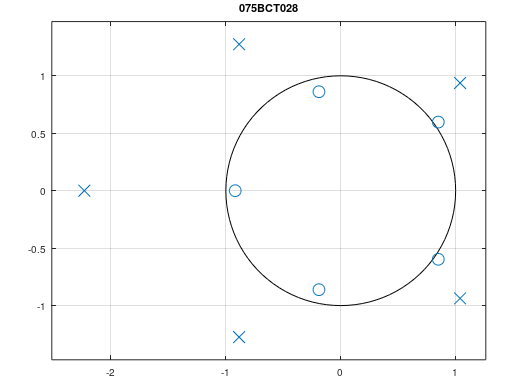
\includegraphics{labss/Lab5_2.PNG}
                \caption{Poles and zeroes for activity 2}
            \end{figure}
\end{enumerate}
\paragraph{Conclusion\\}
In this way "Lab 5 : z-Transformations" was completed with the help of signal package in MATLAB.
For this we plotted a pole-zero plot for a discrete sequence signal and a pole-zero plot for a transfer function.   
\end{document}